\documentclass{article}
\usepackage[utf8]{inputenc}
\usepackage{graphicx}
\usepackage{float}

\title{Yoga82}
\author{Robin Ruland (xxx); Zhao Sun (pz237) }
\date{12 August 2020}

\begin{document}

\maketitle

\section{Introduction}

In this project, we aim to apply what we have learnt in the Deep Vision course to implement an application that could help people self-improve pose alignment in yoga practices. Given a picture of a person doing a yoga pose, the system would use a deep learning classifier to predict the actual pose name. Subsequently, based on this predicted pose class, it would generate a picture of that same person doing the standard pose with ‘corrected’ alignment. By comparing the original pose with the corrected pose, this person could learn to improve his/her yoga pose alignment without a teacher’s supervision.
\newline
\newline
Our project is based on the Yoga-82 dataset, a diverse dataset of 82 complex yoga poses [1] (https://arxiv.org/pdf/2004.10362.pdf). This dataset contains a varying number of images in each class from 64 (minimum) to 1133 (maximum) with an average of 347 images per class. These images contain yoga pose with clean background as well as in the wild (i.e. with random backgrounds in the forest, beach, indoor, etc.). In addition, some images only contain silhouette, sketch, and drawing version of yoga poses. The dataset provides web links of images along with train and test splits. The dataset is released by a group of researchers from Osaka University, Japan, and IIT Gandhinagar, India, in April 2020.


\section{Classification (Robin Ruland)}




\section{Image Generation (Zhao Sun)}

\subsection{Modification from the Original Proposal}

In the original project proposal, we had stated that we wanted to synthesize images based on a Generative Adversarial Network (GAN). However, as we deepened our research on the related works [8,9,10], we realized that the GAN-based proposal is not suitable for our project due to limitations in our chosen dataset. The Yoga82 dataset contains labelled images of yoga poses in the wild; it lacks person re-identification, i.e. it does not have the same person doing different sets of yoga poses. Hence, a discrimination of real (ground truth images) vs fake (synthesized images) is impractical. Subsequently, as we progressed with the Deep Vision course, we were inspired by the last exercise on conditional Variational Autoencoders (VAE) [2] as well as Patrick Esser’s paper on VUNet [1]; we have thus decided to adopt a conditional VAE architecture instead of GAN for the image synthesis part of the project.

\subsection{Objectives and Related Works}
The aim of the generative model is to synthesize an image of a person doing a yoga pose based on an input image of the same person and a label for a target pose. Figure~\ref{fig:schema} illustrates the overall schema. 

\begin{figure}[!h]
    \centering
    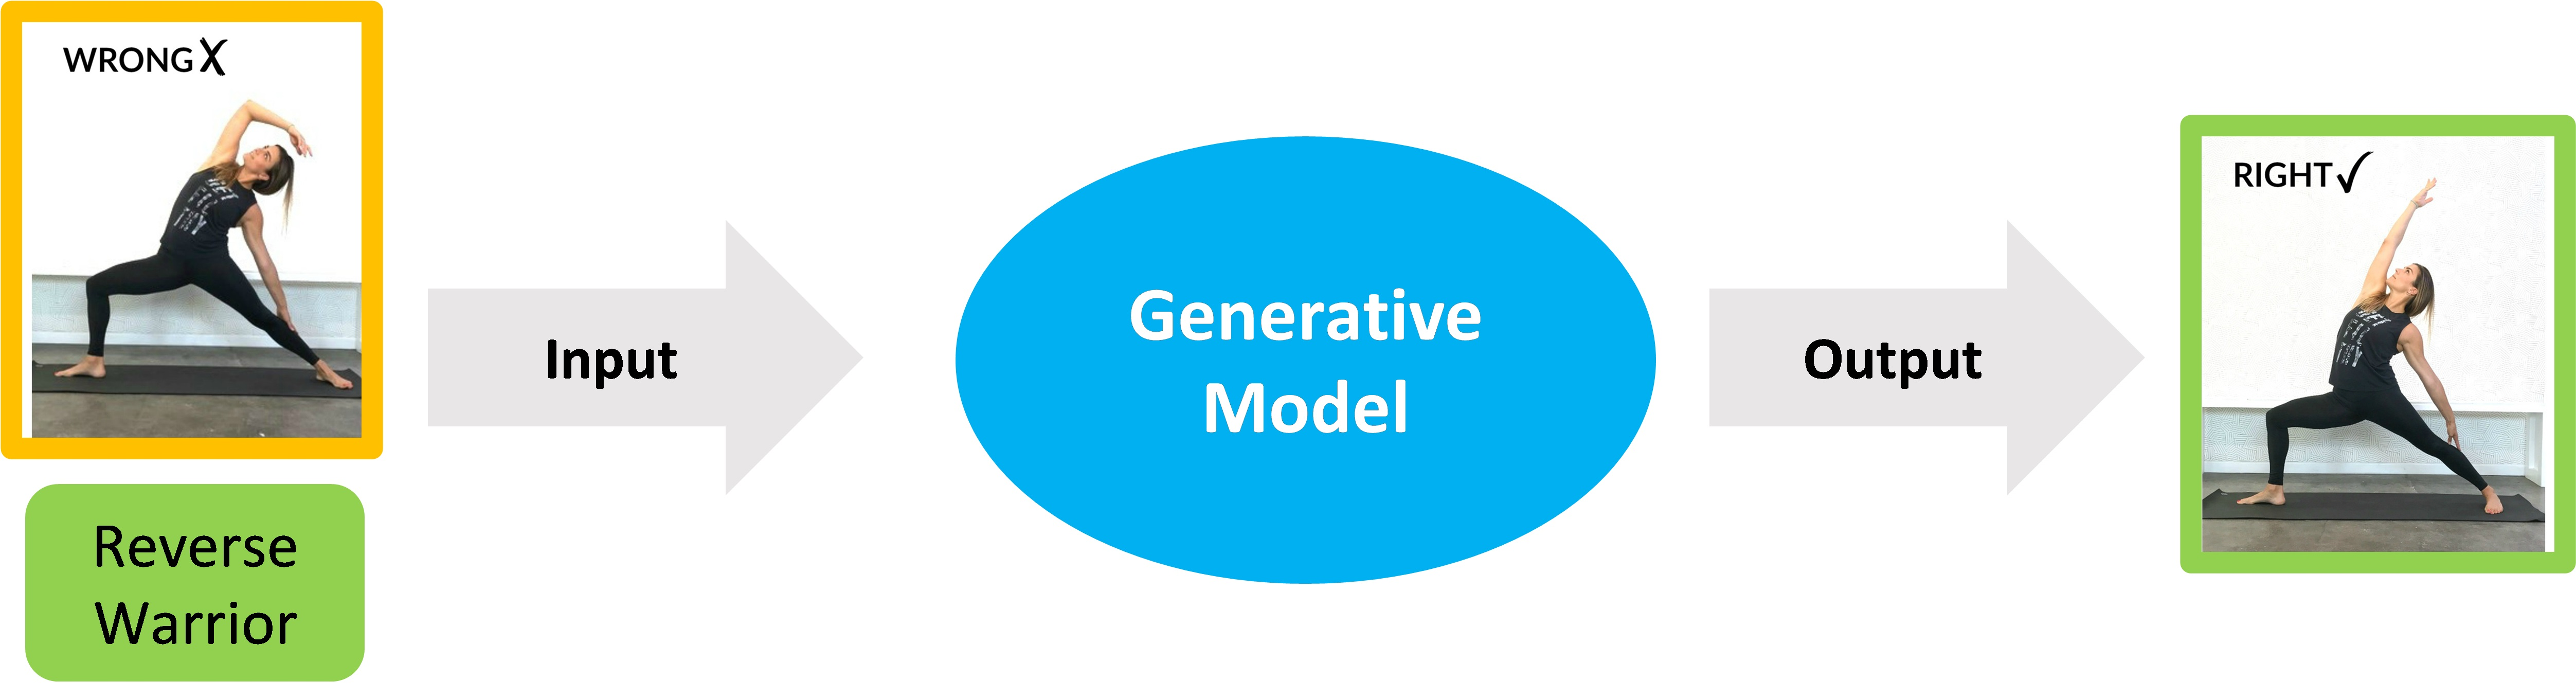
\includegraphics[scale=0.11]{fig1.jpg}
    \caption{The overall schema for yoga pose generation conditioned on a pose label.}
    \label{fig:schema}
\end{figure}

\noindent
In order to achieve this, we can break the task down into several sub-parts: Human Poses Estimation [3,4], Pose Transfer [1,8,10], Text-to-Image Generation [5], etc. While each of the sub-topics is interesting and worth being researched separately, we have, in the interest of time, opted to adapt existing models rather than developing our own end-to-end ones from scratch. For example, the standard off-the-shelf models from the Pytorch library are used for the subtask key points detection and the conventional method of one-hot encoding is applied to convert the text-based pose labels.
\newline
\newline
The key challenge in this project is two-fold: firstly, our model needs to disentangle appearance from pose for an input image; secondly, it needs to learn the association of yoga poses with the respective labels so that it can generate a desired pose conditioned on a given label. We have made a few attempts at different model architectures, as detailed below.


\subsection{Model Architecture I}
This first attempt is based on a combination of VUNet [1] with modifications inspired by the conditional VAE in the Deep Vision Exercise Sheet 10.
\newline

\begin{figure}[H]
    \centering
    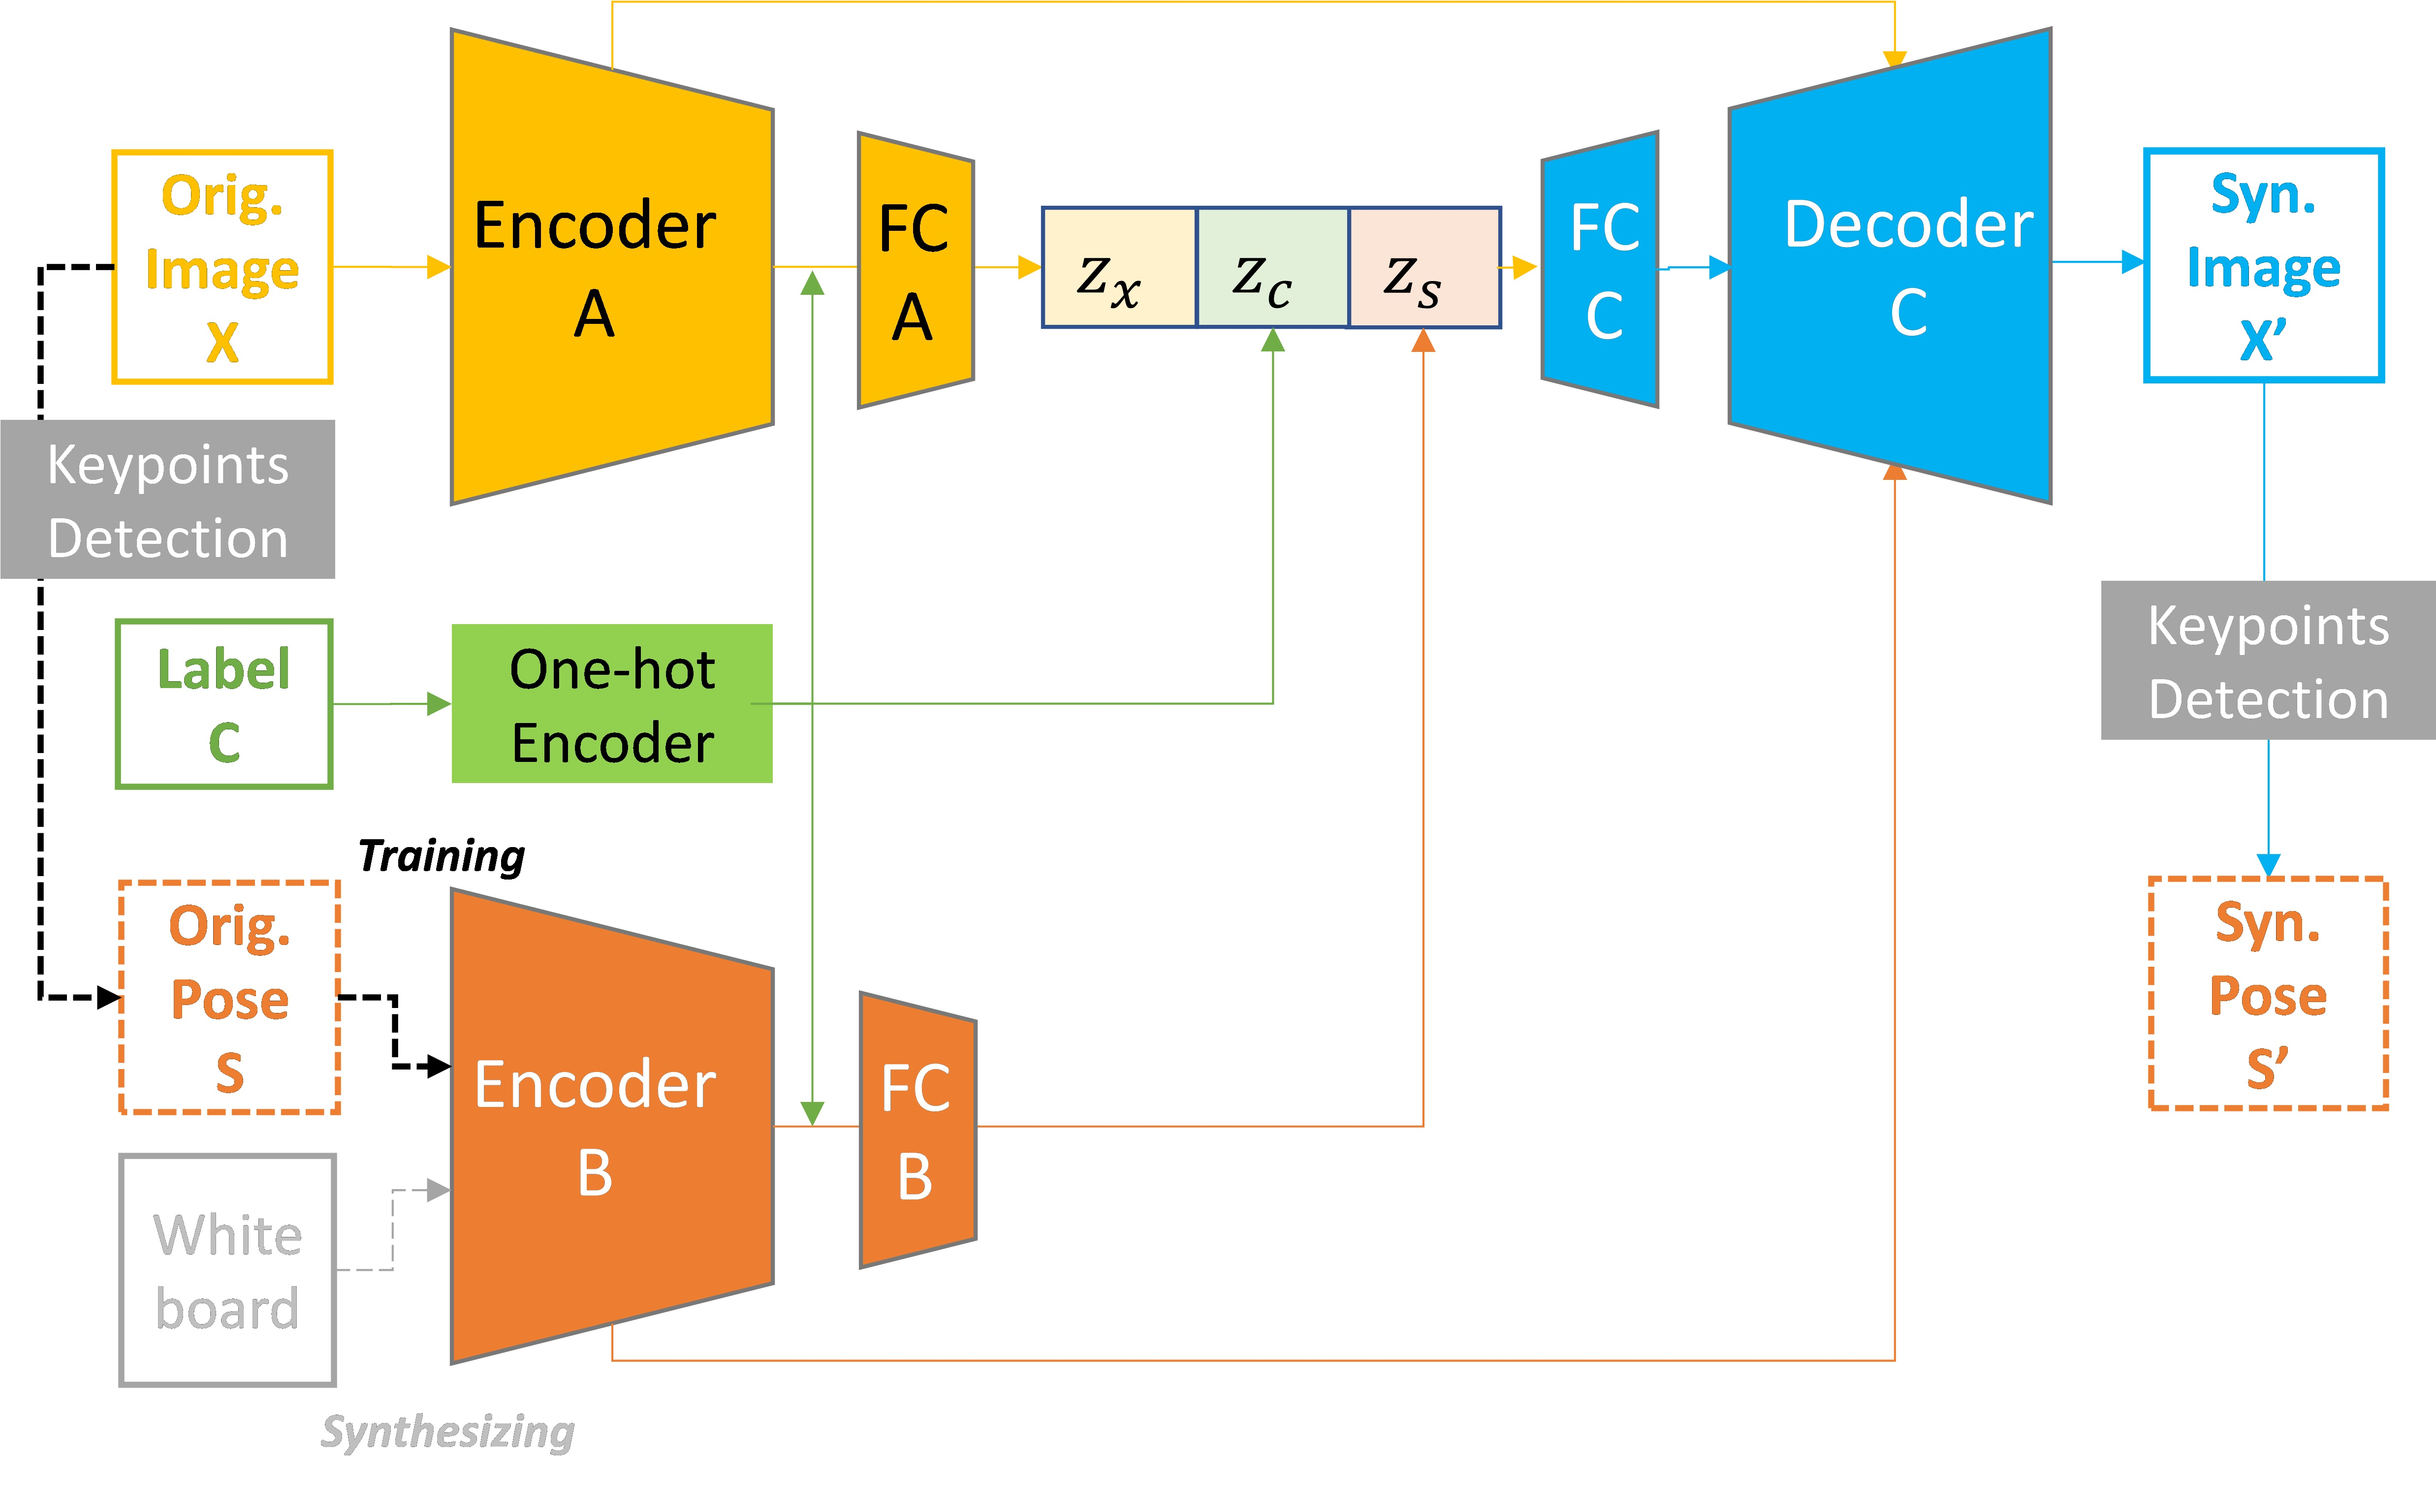
\includegraphics[scale=0.11]{fig2.jpg}
    \caption{Illustration of the schematic diagram on Model Architecture I.}
    \label{fig:arch1}
\end{figure}
\noindent
Overall the model has a joint-UNet structure with two Encoders and one Decoder. Each encoder/decoder unit consists of three residual blocks [6], two downsampling/upsampling layers, and four fully connected layers, respectively. Encoder A takes the original image as input; Encoder B takes the pose estimation as input, which is derived from feeding the original image into a pre-trained key points detection model based on Mask R-CNN ResNet-50 FPN [2]. The text-based pose label is converted via one-hot encoding [5] before feeding into the fully connected layers. Instead of using 82 binary bits to directly encode the corresponding 82 yoga poses in the database, we retain the hierarchical classification structure by using the first 6 bits to represent the Level 1 classification, the next 6 bits to represent the Level 2 classification and the last 8 bits to represent the Level 3 classification. Finally, skip-connections have also been separately established between each encoder and decoder.
\newline
\newline
The intention behind the model design is to represent the yogi’s appearance ${X}$ by latent features ${z_x}$ and the pose shape ${S}$ by latent features ${z_s}$, while simultaneously conditioned on pose label ${C}$ during model training. When synthesizing images, we only need the raw image ${X}$ and pose label ${C}$ as inputs, as we replace the target pose by a ‘whiteboard’ and sampling the latent feature ${z_s}$ at random.
\newline
\newline
\textit{Loss Function}
\newline
\newline
The loss function associated with this model is the sum of the following items:

\begin{itemize}
\item Negative conditional log-likelihood [2], $– log P(X|C) – log P(S|C)$ of image $X$ and pose $S$ given a conditioning $C$, the text-based label in this case. Similar to the approach shown in the lecture, we obtain the evidence lower bound (ELBO):
\begin{figure}[H]
    \centering
    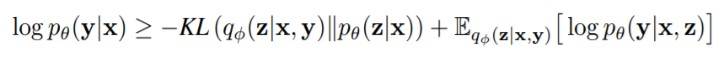
\includegraphics[scale=1]{ELBO.jpg}
\end{figure}
by assuming the latent variables $z_x$ and $z_s$ are statistically independent of input variables $X$ and $S$, i.e. $p(z|x) = p(z)$. By further assuming the priors to be a diagonal unit Gaussian, we can simplify the loss function to be the sum of the negative Kullback–Leibler divergences between the variational posterior and the prior on the latent variable $z_s$ and $z_x$.  
\item Perceptual loss between the original input image X and the reconstructed image X’, which is obtained by adding the content loss and the style loss derived from a VGG19 model [7]
\item Pixelwise MSE Loss between the pose estimation S derived from the original image X and the pose estimation S’ derived from the reconstructed image X’
\end{itemize}

\noindent
\textit{Model inputs}
\begin{itemize}
\item Input image size: 100x100x3
\item Number of model parameters: 2.6M
\item Batch size: 10 [constraint of GPU]
\item Learning rate: 1e-3
\item ADAM optimizer
\end{itemize}

\noindent
\textit{Results Discussion}
\newline
\newline
After training for 5 epochs, we inference from the model to generate the following images:

\begin{figure}[H]
    \centering
    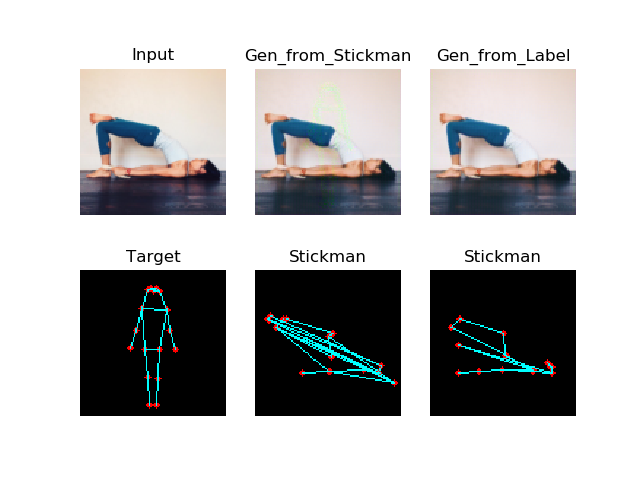
\includegraphics[scale=0.34]{f3.png}
    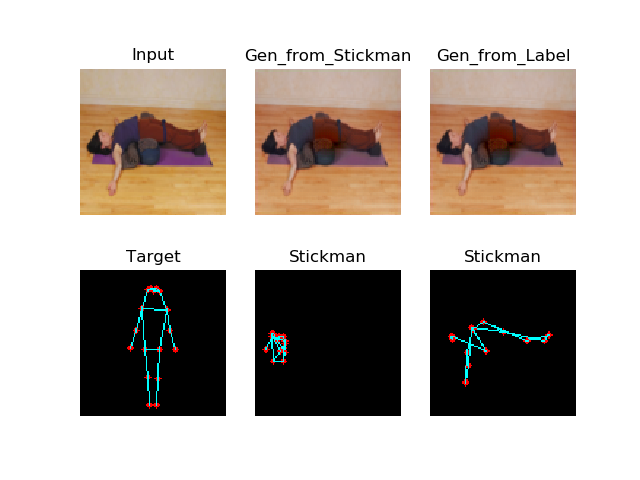
\includegraphics[scale=0.35]{f4.png}
    \caption{Output from Model I}
    %\caption{The first columns show the input images and the target poses; the middle columns demonstrate the synthesized images conditioned on both the target label and pose; the last columns demonstrate the synthesized images conditioned on the target label only. The stickman figures on the bottom are generated from the respective synthesized images.}
\end{figure}

\noindent
The model fails to generate the desired output, i.e. a synthesized image of the input person doing the target pose. Instead, it results in an image of the same person doing the original pose. There are several potential causes for the model failure:

\begin{itemize}
\item The model fails to separate poses from appearances in the feature space, probably due to the design of the network which might require more layers of depth.
\item The conditioning influence from the pose label is too weak, probably due to the limitation of the dataset, i.e. for each pose, the number of images per class varies from 64 to 1133. For such small sample sizes (and without any data augmentation), the model cannot effectively learn to associate pose shapes with labels.
\item The loss function is probably biased towards enforcing the synthesized image to be as similar as possible to the original image, resulting in the skip-connections being over-weighted to channel the original image to the output.
\end{itemize}

\noindent
In addition, the training is extremely slow due to the loss function requiring the reconstructed image to be fed into an external VGG-19 model for perceptual loss calculation as well as the key points detection model for comparing the pixel-wise stickman figures. We have subsequently decided to limit our target poses to only 10 classes, instead of the entire set of 82 classes in the database. We have chosen our yoga classes carefully such that the hierarchical classification structure is retained and well represented.  

\subsection{Model Architecture II}

In the second attempt, we have simplified the model structure to include only one encoder and one decoder. In order to speed up the training time, the encoder now takes a pre-processed image which is a combination of a segmentation layer (blue channel) based on the original image, a key-point layer (red channel) and a stickman layer (green channel) connecting the key joints. This alteration on the input is intended to focus the model on the shape of the human pose in the foreground rather than all the pixels in the background. Like before, our aim is to condition the model on learning various poses associated with the hierarchical class labels. 
\newline
\newline
\noindent
The encoder and decoder have the same basic components as the previous model, with each unit consisting of 3 residual blocks, 2 downsampling/upsampling layers, and 4 fully connected layers, respectively. We attempt to abstractly represent only the yoga pose by superimposing a mask layer on top of the stickman figure, in contrast to considering both appearance and shape in the previous model. The one-hot encoder for the hierarchical class label is kept the same as before, i.e. the conditioning label is fed into the fully connected layers as well as concatenated with the latent features $z_x$ before the decoder. We have experimented with two different versions of design: with skip-connections and without skip-connections between encoder and decoder.

\begin{figure}[H]
    \centering
    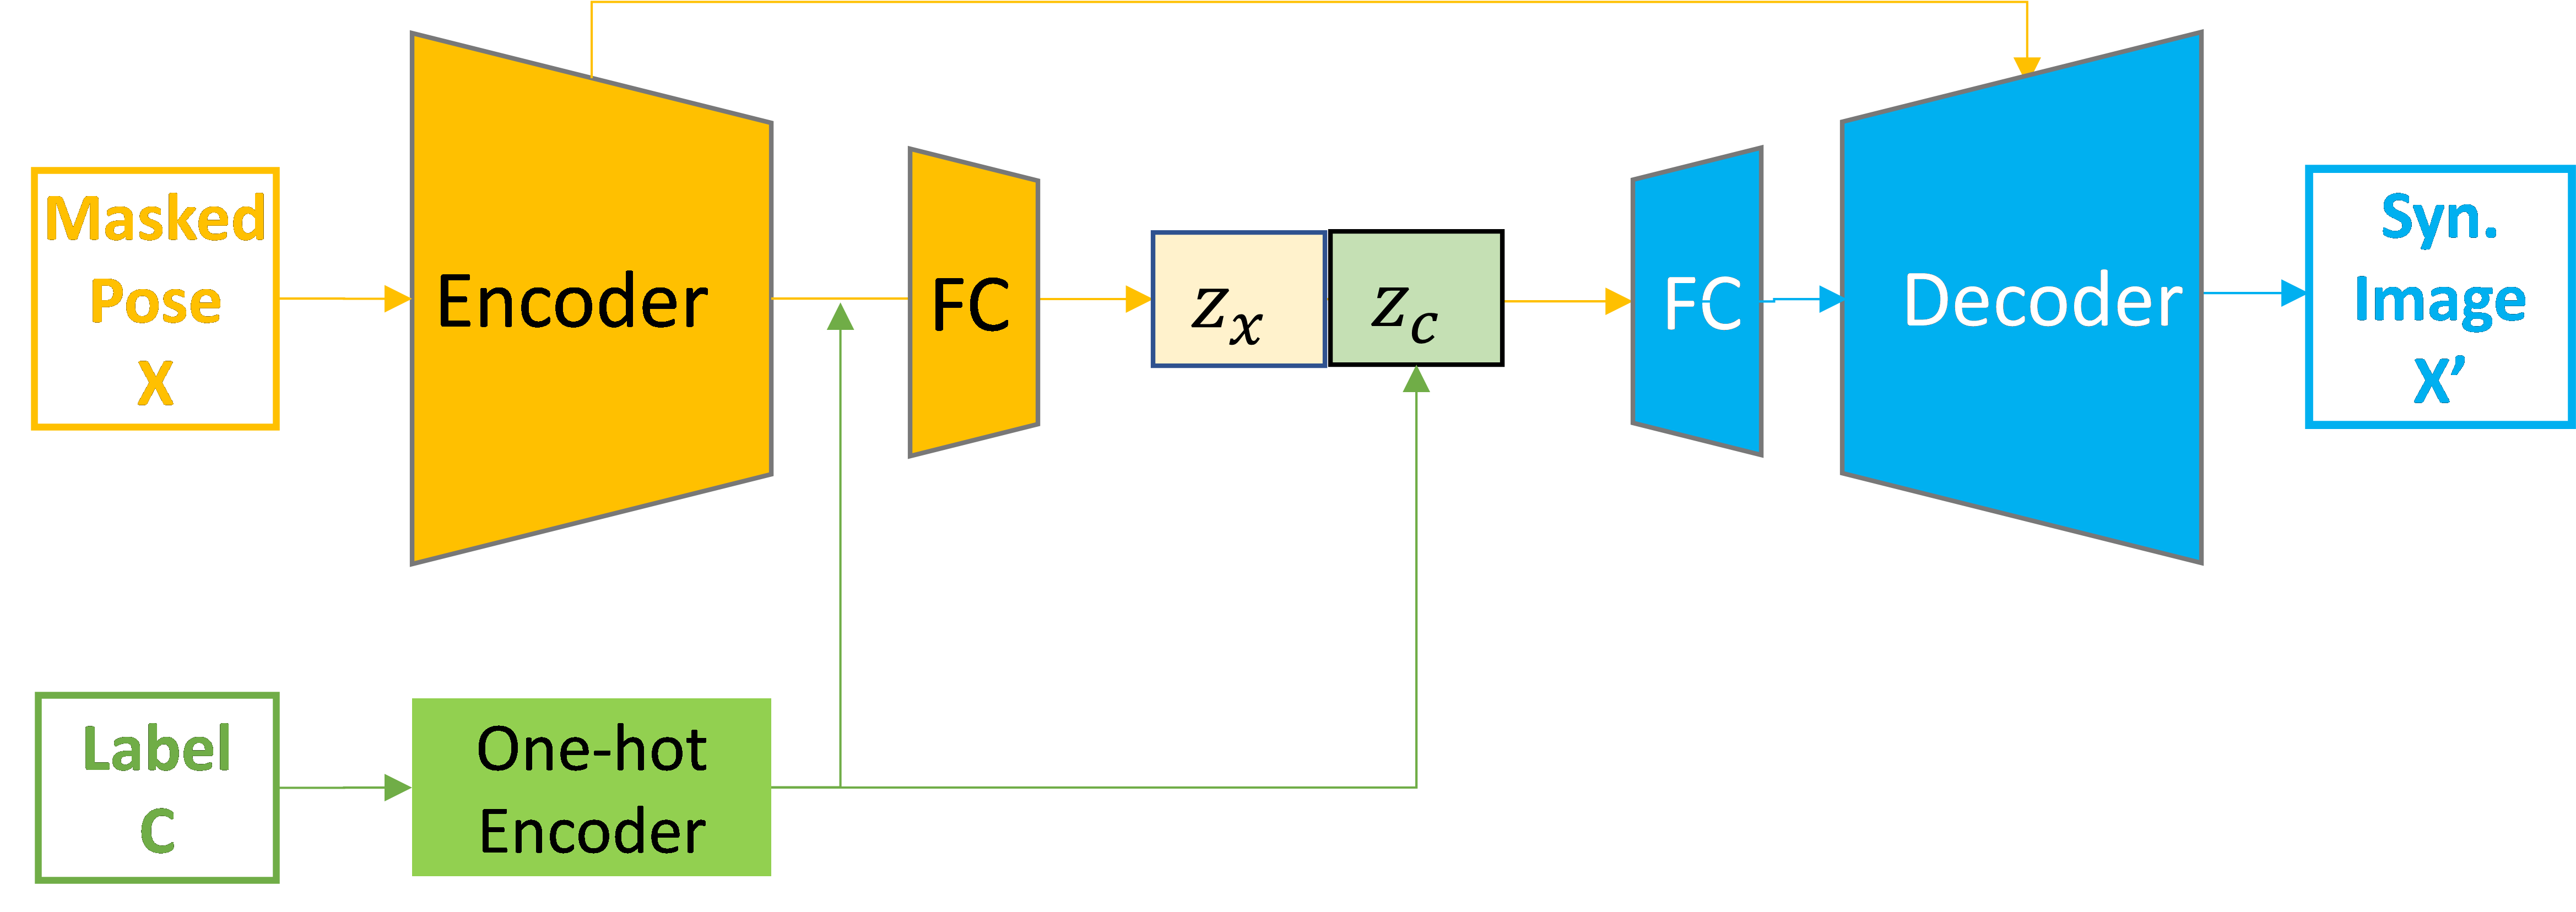
\includegraphics[scale=0.11]{fig4.png}
    \caption{Illustration of the schematic diagram on Model Architecture II.}
\end{figure}

\noindent
\textit{Loss Function}
\newline
\newline
We also further simplified the loss function in order to speed up training. The loss function now only includes two items:

\begin{itemize}
\item Negative Kullback–Leibler divergence between the posterior and the prior on the latent variable $z_x$, assuming the prior to be a diagonal unit Gaussian
\item Pixelwise MSE Loss between the synthesized image and the input
\end{itemize}

\noindent
\textit{Model inputs}
\begin{itemize}
\item Input image size: 100x100x3
\item Number of model parameters: 1.9M
\item Batch size: 32 [constraint of GPU]
\item Learning rate: 1e-3
\item ADAM optimizer
\end{itemize}

\noindent
\textit{Results Discussion}
\newline
\newline
After training for 20 epochs, we inference from the model to generate the following images:

\begin{figure}[H]
    \centering
    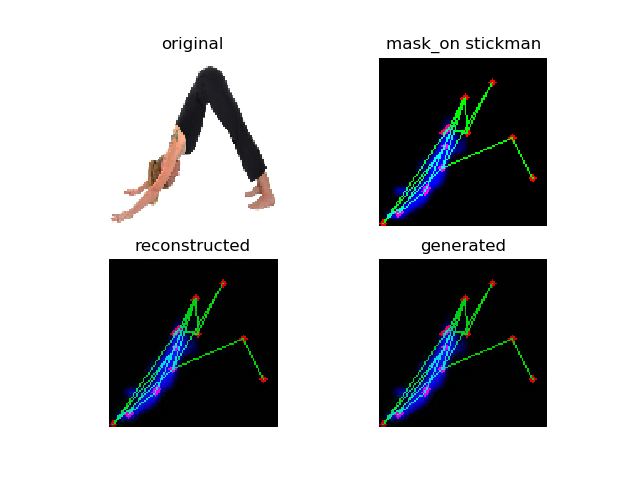
\includegraphics[scale=0.36]{f5.png}
    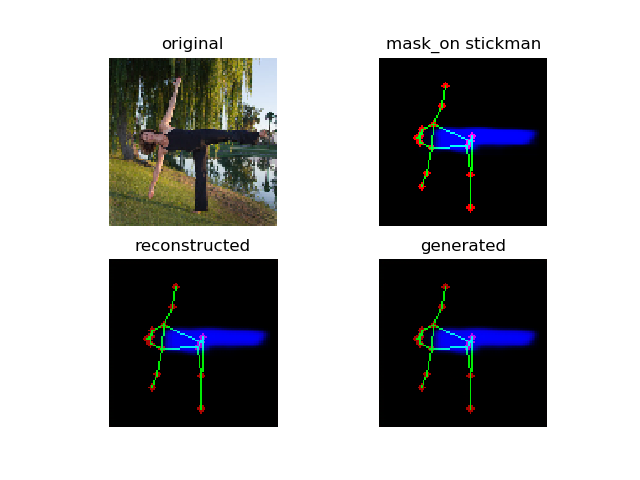
\includegraphics[scale=0.36]{f6.png}
    \caption{the top row shows the original image and the pre-processed input image consisting of a mask layer on the key points and stickman figure; the bottom row shows the reconstructed image and the generated image.}
\end{figure}

\noindent
This simplified model again does not generate the desired output, i.e. we failed to condition the model on the pose label. Like before, the output is exactly like the input image. This is probably due to the presence of the skip-connections that the model just learned to transfer the input image directly into the output image. Furthermore, in order to test our hypothesis on the skip-connections, we have tested the model with the skip-connections removed. We have also experimented with replacing MSE loss with L1 loss for the pixel by pixel comparison.
\begin{figure}[H]
    \centering
    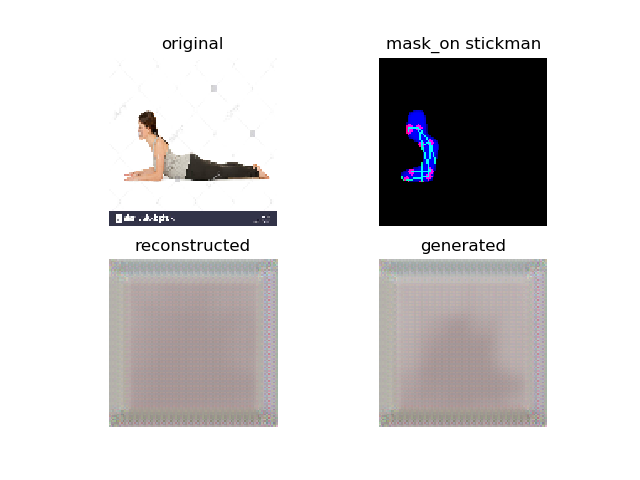
\includegraphics[scale=0.36]{f7.png}
    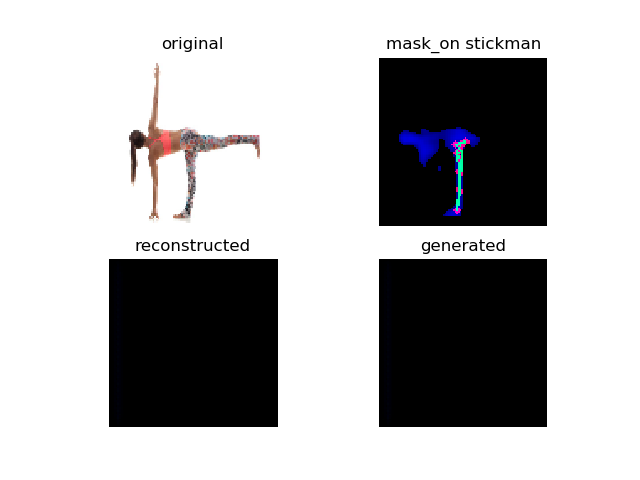
\includegraphics[scale=0.36]{f8.png}
    \caption{Results from removing skip-connections from the model; the 4 images on the left are the experimental results under MSE loss; the 4 images on the right are associated with L1 loss.}
\end{figure}

\noindent
Notice the inaccuracies associated with the mask and key points detection generated from the original image by the pre-trained models. These are probably due to the inherent limitation of the yoga82 dataset, which might also contribute to the failure of the model to separate the poses conditioned on the label. 

\subsection{Reflections and Possible Future Work}

We originally aimed to generate standard yoga poses with correct alignment from an input image with misaligned posture. However, we faced the following limitations:

\begin{enumerate}
\item The accuracy of the Pytorch pre-trained key points detection model for human pose estimation is low for the Yoga82 dataset. 
\item We cannot train our own pose estimation model due to the lack of key-point ground truth labelling in the Yoga82 dataset. 
\item The Pytorch segmentation model for the mask layer is similarly dysfunctional when applied to the Yoga82 dataset.
\item The above limitations in input quality render loss function optimization during training futile (garbage-in garbage-out).  
\end{enumerate}

\noindent
In the future, we would greatly benefit from a better suited dataset, that should include multiple sets of yoga poses performed by the same set of persons, preferably with labelled body parts.  We could further enlarge the training dataset via data augmentation. We need a better model to generate sensible human stick figures and masks. Moreover, an advanced future target would be to incorporate video streams of people doing yoga. This would provide greater scope to train the model as each video frame would not only provide incremental example poses, but also the graph of pose transformations necessary to more accurately generate pose images or video. 


\section{References}
\textit{Image Generation}
\begin{enumerate}
\item Esser, et al. A Variational U-Net for Conditional Appearance and Shape Generation. (2018)
\item Sohn, et al. Learning Structured Output Representation using Deep Conditional Generative Models (2015)
\item He, et al. Mask R-CNN (2018)
\item Cao, et al. Realtime Multi-Person 2D Pose Estimation using Part Affinity Fields. (2017)
\item Reed, et al. Generative Adversarial Text to Image Synthesis. (2016) 
\item He, et al. Identity Mappings in Deep Residual Networks. (2016)
\item Johnson, et al. Perceptual Losses for Real-Time Style Transfer and Super-Resolution (2016)
\item Siarohin, et al. Appearance and Pose-Conditioned Human Image Generation using Deformable GANs (2019)
\item Zhu, et al. Progressive Pose Attention Transfer for Person Image Generation (2019)
\item Ma, et al. Pose Guided Person Image Generation (2017)
\end{enumerate}



\end{document}